\chapter{Amélioration - Automatisé, Générique, Open Source et dans le Cloud}

  \section{Les objectifs de cette nouvelle plate-forme d'Intégration Continue}
  Une PIC unique.\\
  Essor du blockchain.\\
  Gouverné par les acteurs du projets. (et non pas AXA Tech)\\

  \section{Le serveur d’Intégration Continue}
  Afin de répondre à la problématique de la généricité de la plate-forme d'Intégration Continue et de l'open source le serveur d'Intégration Continue devra répondre des caractéristiques suivantes:\\

  \begin{itemize}
    \item multiplate-forme (Windows et Linux),
    \item multi-langage (.NET, JAVA/J2EE, Javascript, ...),
    \item multi-référentiel de code source (Git, TFS, SVN, ...),
    \item open source.\\
  \end{itemize}

    \subsection{Jenkins leader mais ...}
    Jenkins (ex Hudson) est le leader des serveurs d'Intégration Continue. Développé en Java et sous licence Apache il répond aux caractéristiques vu précedemment. Cependant notre choix ne se portera pas sur lui.

    Jenkins est mal adapté au pipeline de déploiement (Voir la section~\ref{DeployementPipeline}). Il n’a pas été modélisé pour être « First Class »\footnote{First Class: désigne dans les langages de programmation le fait que l'on peut manipuler des fonctions comme n'importe quel objet.}, ce qui implique qu'un « job » ne peut prendre en entrée ou avoir comme sortie un autre job. Il existe des plugins pour palier en partie au manque de cette fonctionnalité mais ils ne semblent jamais fonctionner correctement. Bien entendu nous pouvons définir des « jobs » qui s’exécuteront avant ou après tel autre « job » mais cela est sujet aux erreurs lors de séquences complexes.\footnote{Note de l'auteur: Jenkins 2.0 (en cours de développement lors de l'écriture de ce mémoire) supporte le « first class ».}\\

    Jenkins est un serveur d’Intégration Continue orienté technique. De nombreuses configurations se font par de petits scripts shell coller dans des petites zones de texte et par une profusion de plugins. Son expérience utilisateur (UX), très peu développée n’offre pas de vision claire aux non-initiés. Par exemple, pour afficher le journal de sortie d’une build échoué dans Jenkins peut demander jusqu’à trois clics à partir de la page d’accueil. Cette orientation technique dessert plutôt mal un des principes fondamental du pipeline de déploiement qu’est la collaboration entre les différentes entités impliquées dans le projet. Dans une optique agile et DevOps, où le développeur tente de se rapprocher du métier et des opérationnels en exposant l’avancé de ses développements au jour le jour Jenkins se pose en frein.\\

    \subsection{Visual Studio Team Services}

    \subsection{GoCD, l'alternative}
    GoCD est un serveur d'Intégration Continue spécialisée dans la modélisation et la visualisation de workflow avancée. Multiplate-forme, multilangage, multi-référentiel de code source et open source, GoCD est développé en Java par ThoughtWorks. Sa puissance repose sur son principe de pipeline de déploiement. Rapellons-nous la définition donnée par Martin Fowler:\\

    \begin{quotation}
      \emph{« A deployment pipeline is a way to deal with this by breaking up your build into stages […] to detect any changes that will lead to problems in production. These can include performance, security, or usability issues […] should enable collaboration between the various groups involved in delivering software and provide everyone visibility about the flow of changes in the system, together with a thorough audit trail. »}
    \end{quotation}

    \subsubsection{Le pipeline de déploiement, le succès de GoCD}
    Le séquençage du cycle naturel du Déploiement Continue en pipeline permet de trouver et supprimer les erreurs plus efficacement. Cela absout l'intégration de scripts monolithiques inflexibles, de tests séquentiels lents, de worflows plat et simpliste ... Le raccourcissement des boucles de rétroaction et la répétabilité des tâches automatisées nous permet de traquer facilement les problèmes. De plus la visualisation du processus de Déploiement Continue en un graphe fini améliore la collaboration des différentes équipes travaillant sur le projet favorisant l'apport de valeur (logiciel) aux utilisateurs (production).\\

    \subsubsection{La puissance de l'abstraction de GoCD}
    Selon Barbara Liskov dans sa conférence « The Power of Abstraction » \cite{Lis09} un design logiciel est bon quand de puissante abstraction simple rendent un problème complexe traitable. GoCD repose sur un principe d'abstraction qui s'articule autours de quatre abstractions et leur relation que sont les Tâches inclues dans les Jobs inclus dans les Stages inclus dans les Pipelines (Voir figure \ref{Pipeline}).\\

    \begin{figure}
      \begin{center}
        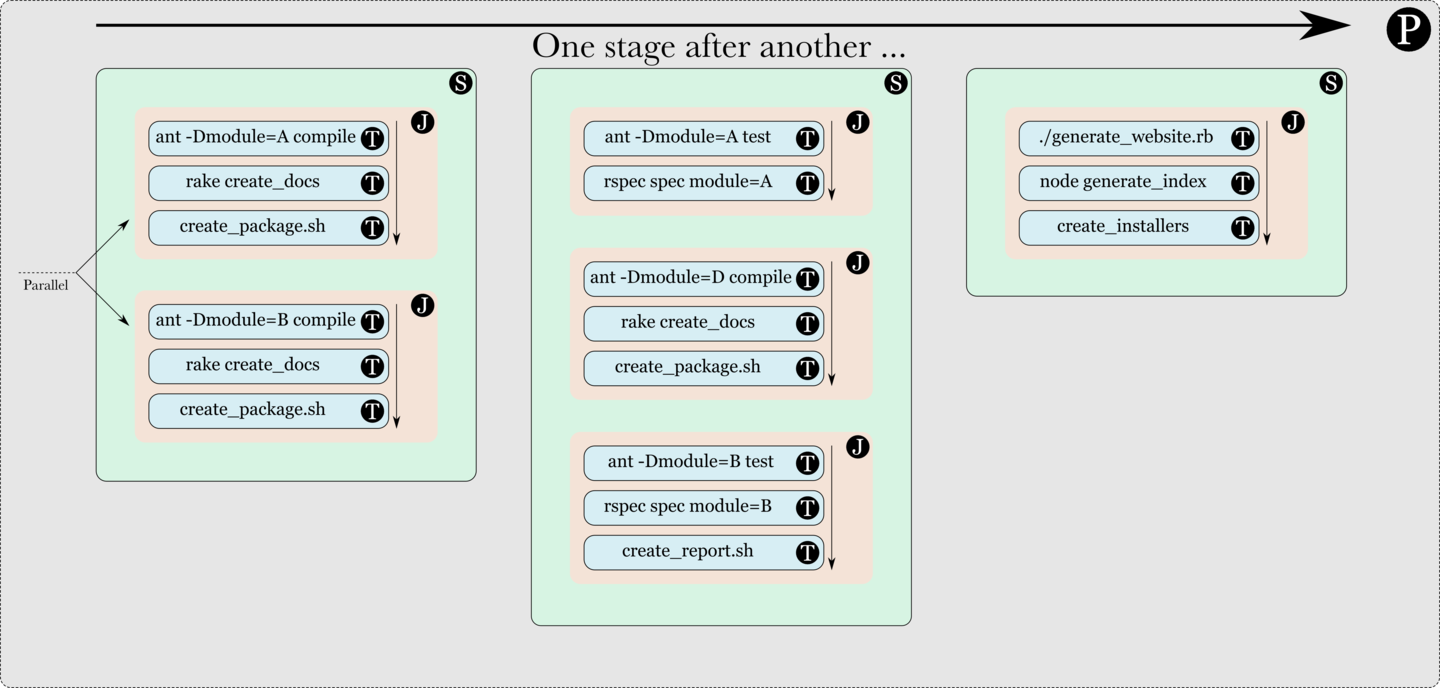
\includegraphics[scale=0.7]{images/pipeline.png}
      \end{center}
      \caption{Schéma du principe d'abstraction de GoCD}
      \label{Pipeline}
    \end{figure}

    Il est dès lors trivial de définir différents triggers (déclencheurs) de comportements pour les Pipelines et les Stages. Si nous avions seulement les deux abstractions Jobs et Stages (comme c'est le cas dans Jenkins par exemple) notre Intégration Continue serait surchagée par les différentes configurations des comportements en fonction des différents contextes.\\

    De plus les Jobs et Stages de GoCD sont des primitives, ce qui inclu qu'ils peuvent, et doivent d'être étendus afin d'obtenir des abstractions de meilleures ordres.\\

    La puissance de cette abstraction réside dans ses éxecutions parallèles et séquentielles:\\

    \begin{enumerate}
      \item de multiple Pipelines peuvent s'exécuter en parallèle,
      \item les multiple Stages d'un Pipeline s'exécutent séquentiellement,
      \item les multiple Jobs d'un Stage s'exécutent en parallèle,
      \item les multiples Tâches dans un Job s'exécutent séquentiellement.\\
    \end{enumerate}

    Ce comportement d'exécution alternées a été délibérement conçu par ThoughtWorks de sorte que nous ayons la possibilité de paralléliser et séquentialiser notre worklow selon ces deux niveaux de granularité.

    \subsubsection{Le concept de First Class au service du pipeline de déploiement de GoCD}
    Le fait que l'on puisse manipuler les abstractions de GoCD comme des fonctions permet de:\\

    \begin{enumerate}
      \item déclencher un Pipeline comme un unité,
      \item faire qu'une Pipeline dépende d'une ou plusieurs autres,
      \item faire traverser des artefacts au travers d'un Pipeline,
      \item avoir le contrôle d'accès au niveau d'un Pipeline,
      \item associer des Pipelines à des environnements,
      \item comparer les changements entre deux instances d'un Pipeline.\\
    \end{enumerate}

    Le pipeline de déploiement peut ainsi dépendre, en entrée, de plusieurs autres Pipeline (fan-in) et de déboucher sur l'exécution de plusieurs autres Pipeline (fan-out) (Voir Figure \ref{VSM}).

    \begin{figure}
      \begin{center}
        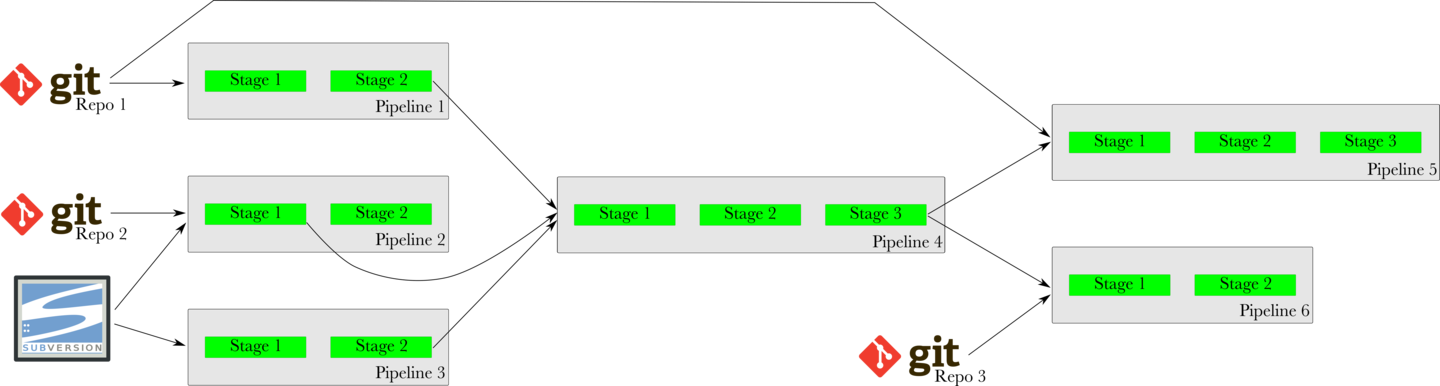
\includegraphics[scale=0.7]{images/VSM.png}
      \end{center}
      \caption{Schéma d'une séquence de Pipelines}
      \label{VSM}
    \end{figure}

    \section{Le référentiel de code source}\label{Repository}
    GoCD intègre parfaitement les divers référentiels de code source. Des agents ont été développé par ThoughtWorks et la communauté de GoCD pour les principaux référentiels de code source (TFS, Git, Github, SVN, Mercurial). De plus GoCD offre la possiblité aux utilisateurs d'utiliser les Webhooks\footnote{Les webhooks servent à notifier des éléments externes à une application web qu'un événement a eu lieu sur celle-ci.} afin de notifier le serveur d'Intégration Continue qu'une modification a été apporté aux code source.\\

    Le choix du référentiel de code source dépend essentiellement de la politique interne du versionning de votre entreprise. Dans la suite de ce mémoire nous utiliserons Github comme référentiel de contrôle pour notre plate-forme d'Intégration Continue.

      \subsection{Github}
      Github est un service web d'hébergement et de gestion de code source propriétaire. Cela enfreint un des invariants de notre plate-forme vu précédemment qu'est la qualité open source de notre projet me direz-vous. Certe. Cependant Github n'est qu'une surcouche service au gestionnaire de version Git, qui lui est open-source (Linux - Licence GNU). Pour faire simple Github offre une interface utilisateur et un hébergement dans le cloud à Git.

      Le choix de Github pour cette PIC est simplement dû à une contrainte temporelle. Des alternatives open source sont disponnible sur internet (Gogs, Phabricator, GitBucket) et pourraient être hébergés sur notre serveur d'Intégration Continue. Cepandant Github étant la référence mondiale des référentiels de code source, la plupart des plugins utiles à la réalisation de notre PIC ont déjà été développés par la communauté. Ce qui facilitera la mise en place expérimentale de notre serveur d'Intégration Continue.

    \section{Configuration de GoCD}
    La polyvalence d'une plate-forme d'Intégration, outre le choix des outils, réside dans sa configuration. Parfois complexe et fastidieuse la configuration du serveur peut rebuter certains développeurs. Pourtant une fois maîtrisée et mise en place, les gains apportés par l'Intégration Continue sont non négligeables. Nous allons tenter d'illuster le pipeline de déploiement d'un projet classique composé d'une unique application.

      \subsection{Configuration générale}
      Après installation du serveur GoCD, pour un usage classique, aucune configuration n'est nécessaire (selon la documentation officielle). GoCD se veut facile d'installation, de configuration et d'utilisation. Cependant je vous conseille fortement de paramétrer la gestion des artefacts ainsi que la sécurité au niveau des accès.

        \subsubsection{La gestion des artefacts}
        Il est fortement conseillé, et ce pour n'importe quel serveur d'Intégration Continue, de créer une partition séparée et extensible sur votre serveur ou dans votre infrastructure pour les artefacts créés. Le dêpot d'artefact peut croître en taille très rapidemment. S'il est situé sur la partition principale de votre système, vous pourriez rencontrer des problèmes de perte de données ou de comportement du serveur dans le cas ou le disque serait plein.

        \subsubsection{La gestion des accès}
        Le serveur d'Intégration Continue étant au centre de votre développement, doit être régi par une politique d'habilitation afin d'éviter tout problème de disfonctionnement lié à une erreur utilisateur. Les fonctionnalités de gestion des utilisateurs de GoCD vous permettent de contrôler l'accès à votre serveur via un principe d'autorisation basé sur un mécanisme de rôle. Les rôles regroupent un ensemble d'utilisateurs, avec des activités fonctionnelles similaires, et leur accordent un ensemble commun d'habilitation.

      \subsection{Création d'un pipeline de déploiement et de notre premier Stage, la « build »}
      La première étape à effectuer dans la configuration d'un processus d'Intégration Continue et de déploiement de GoCD est de créer un nouveau Pipeline pour notre application. L'interface graphique de GoCD nous propose de faire cela en trois étapes. La première, appelée « Basic Settings » définie le nom de notre Pipeline ainsi que son groupe dans le cas d'un projet multi-applicatifions ou d'une organisation particulière.\\

      La deuxième étape, appelé « Material » permet de définir le point d'entrée de votre Pipeline. Le Material peut-être notre gestionnaire de code source, un package repository (dêpot de binaires) ou encore un autre Pipeline (First Class). Dans notre cas nous choisissons de spécifier en point d'entrée notre réferentiel de code source. Pour cela nous sélectionnons le Material « Git », indiquons l'URL du repository Github correspondant à la branche de notre application que nous souhaitons automatiser et définissons la stratégie d'orchestration de notre serveur (Voir la section \ref{ServeurCI}).\\

      La troisième et dernière étape à prendre en compte lors de la mise en place d'un Pipeline est la création de notre tout premier Stage. Cette dernière peut être effectuée manuellement - dans le cadre d'un tout nouveau type de Stage - ou via le biais d'un template prédéfini - rappelons que toutes les configurations de GoCD sont stockées au format XML et donc réutilisables. Ne disposant pas encore d'autre Stage, nous réalisons la configuration de notre Stage de « build » manuellement. Pour cela nous lui donnons un nom et définissons son type de déclenchement; « On Success » dans le cas d'un trigger automatique basé sur la réussite du Material ou « Manual ». Dans le cas d'une Intégration Continue optimale toutes les actions de cette dernière doivent être automatiser, nous nous tournons donc vers le déclenchement « On Success ». La suite de cette étape de création de Stage est d'initialiser un Job, en lui donnant un nom et une Task en définissant son type - Ant pour le Java, NAnt pour le .Net, Rake pour le Ruby... - et le son répertoire de travail. Dans le cas ou aucun type ne correspond à votre besoin vous pouvez directement taper votre ligne de commande.\\

      Nous venons de construire notre premier pipeline composé d'un Stage de build exécuté à chaque commit sur Github.

      \subsection{Les tests}
      A ce stade, notre processus d'Intégration Continue est très sommaire, il effectue exclusivement que la build de notre code source. L'étape suivante est d'automatiser l'ensemble de nos tests après chaque build. Pour cela nous allons mettre en place un nouveau Stage composé d'un ensemble de Jobs chargés d'exécuter nos différents tests (tests unitaires, tests d'intégration, tests fonctionnelles, ...).\\

      Afin d'exécuter nos tests, deux options s'offrent à nous. Nous pouvons utiliser les frameworks propres à chacun et générer des rapports au format XML ou utiliser Gauge, un outil développé par Thoughtworks (à l'origine du développement de GoCD). Bien qu'attrayant, Gauge n'est encore que trop limité au niveau de ses plugins ne se couple pas avec tous les frameworks de test disponibles. Cependant, GoCD intègre l'agent Gauge Report permettant de visualiser graphiquement les fichiers de sorties des tests aux formats XML. L'exécution des tests sera donc automatisé par ligne de commande et reporté graphiquement via l'interface du site web (Voir la figure \ref{GoCDReportTest}).\\

      Nous définissons donc un nouveau Stage qui sera composé d'autant de Jobs que de types de tests effectués. Chaque Job pourra contenir une ou plusieurs tasks en fonction de votre découpage. Le déclencheur de ce Stage de test sera le succès du Stage de build.

      \begin{figure}
        \begin{center}
          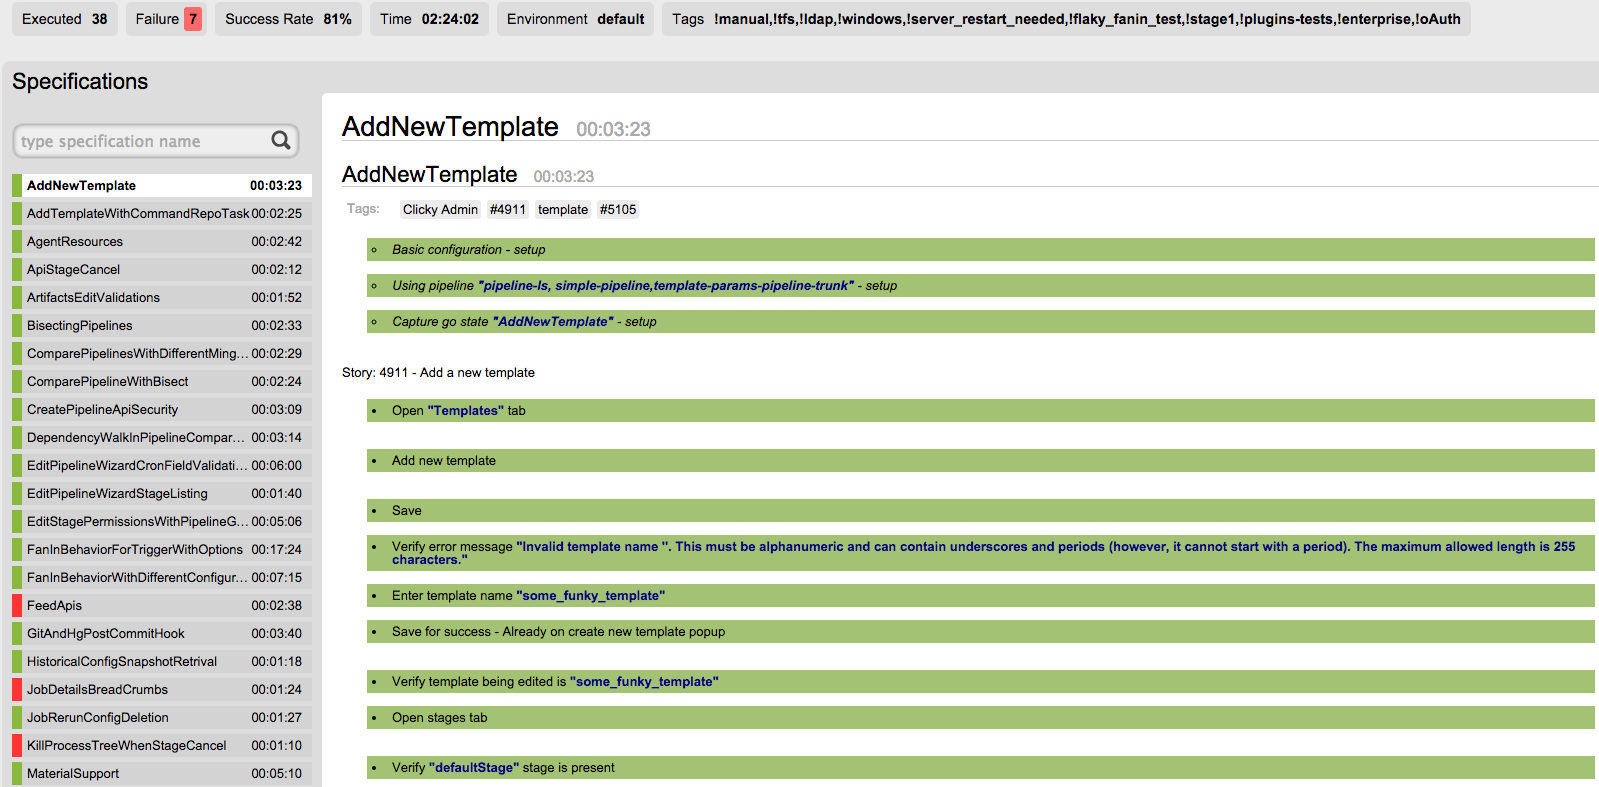
\includegraphics[scale=0.15]{images/GoCDReportTest.png}
        \end{center}
        \caption{Visualisation d'un rapport de test dans GoCD}
        \label{GoCDReportTest}
      \end{figure}

      \subsection{L'inspection du code}
      L'inspection statique du code source est une étape majeure dans l'assurance qualité de l'Intégration Continue. Déjà présent et configurée au sein des pipelines de déploiement des projets AXA via l'outil SonarQube nous allons l'intégrer au sein de notre PIC. Reprenons notre configuration illustrative d'un Pipeline de déploiement classique; elle contient actuellement le Stage de build et le Stage de test. L'inspection de code source se situe en amont de la build. Nous allons donc créer un nouveau Stage qui prendra en Material le gestionnaire de code source et qui sera le Material du Stage de build. Ce Stage sera chargé d'exécuter SonarQube et d'enregister le rapport au format HTML pour qu'il puisse être affiché par un agent de GoCD (Voir la figure \ref{GoCDSonar}).\\

      \begin{figure}
        \begin{center}
          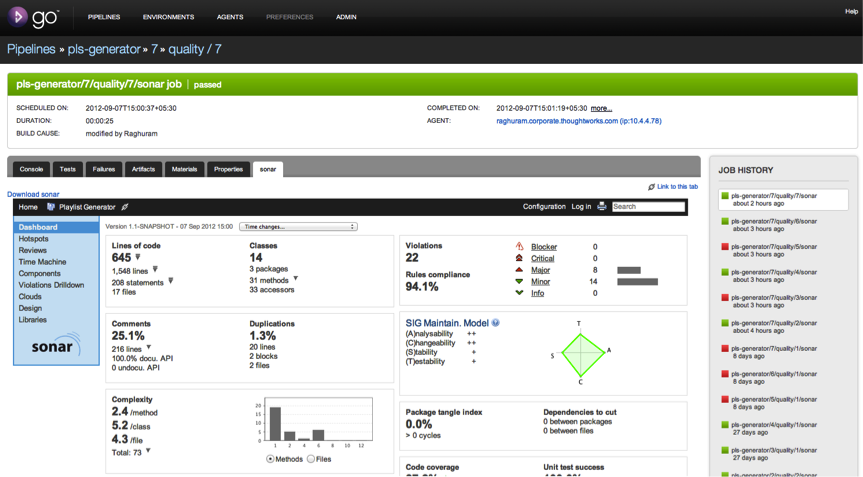
\includegraphics[scale=0.7]{images/GoCDSonar.png}
        \end{center}
        \caption{Visualisation d'un rapport d'analyse statique de code dans GoCD}
        \label{GoCDSonar}
      \end{figure}

      \subsection{La documentation}

      \subsection{Architecture et fonctionnement de la PIC}
      A ce stade du mémoire notre Plate-forme d'Intégration Continue est hébergée sur un serveur interne physique. Notre référentiel de code source, hébergé par Github, repose sur l'approche du « post commit hook » (Voir la section~\ref{ServeurCI}). Lorsqu'un développeur pousse son code sur Github, le gestionnaire de code source notifie le serveur d'Intégration Continue qui déclenche l'exécution de son pipeline de déploiement. Les utilisateurs peuvent visualiser l'avancement de leur Intégration Continue sur l'interface web de GoCD (Voir Figure \ref{PICv1}).\\

      L'installation, la configuration et la maintenance de notre PIC est pour l'heure entièrement manuelle.\\

      \begin{figure}
        \begin{center}
          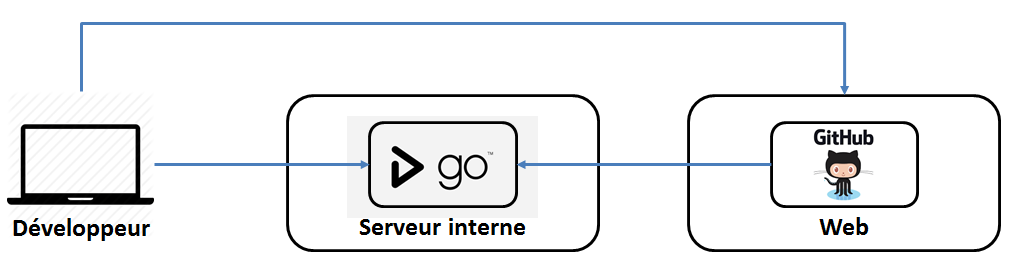
\includegraphics[scale=0.5]{images/PICv1.png}
        \end{center}
        \caption{Schéma de la première version de notre PIC - Standard}
        \label{PICv1}
      \end{figure}

    \section{Migration de la plate-forme d'Intégration Continue dans le Cloud public}
    Le Cloud Computing a récemment émergé comme un nouveau paradigme pour l'hébergement et la prestation de services sur Internet. Il est attrayant pour les entreprises car il élimine la nécessité pour les utilisateurs de planifier à l'avance l'approvisionnement des serveurs et permet aux entreprises de commencer avec de petites ressources pour les augmenter en fonction de la demande. En dépit du fait que le Cloud Computing offre d'énormes possibilités pour l'industrie informatique, le développement de ses technologies et ses utilisations est actuellement à ses débuts.

      \subsection{La valeur ajoutée}
        \subsubsection{L'Agilité}
        Le Cloud Computing accélère et simplifie le provisionnement et les réallocation des ressources de l'infrastructure informatique. Selon nos besoins nous pourront mettre en oeuvre de nouvelles applications, modifier la structure de l'infrastructures, ou augmenter/réduire l'utilisation de nos ressources afin d'améliorer notre Intégration Continue. De plus notre serveur d'Intégration Continue sera accessible hors du domaine réseau d'AXA, offrant ainsi une plus grande mobilité aux équipes de développement.

        \subsubsection{La scalabilité}
        La puissance de traitement des charges de travail de notre serveur d'Intégration Continue fluctue en fonction du temps, des actions et des projets. Une plus grande puissance est requise lors de l'exécution d'un pipeline de déploiement que lors d'une simple visualisation de l'état de nos différentes builds par exemple. C'est ce que l'on appelle scalabilité de l'infrastructure. L'infrastructure de type Cloud adapte la capacité et le nombre de serveurs aux besoins réels tandis que les infrastructures traditionnelles sont conçues pour répondre aux besoins lors des périodes d'utilisation intensive.

        \subsubsection{Les coûts}
        Les ressources Cloud fonctionnent sur le principe du service à la demande. Les entreprises ne paient que ce qu'elles consomment. Les besoins en ressource d'une PIC varient en fonction du cycle de développement des projets présents. Couplé au principe de la scalabilité, la migration de notre serveur d'Intégration Continue dans le Cloud nous permet de reduire notre budget assigné à l'infrastructure.

        \subsubsection{La fiabilité et les sinistres}
        Les fournisseurs de Cloud, intègre à leur plate-forme des mécanismes de migration dynamique, de migration du stockage, de tolérance aux pannes (haute disponibilité) et de plannification des ressources distribuées. Ces fonctionnalités accroissnet le temps de disponibilité et accélèrent les procédures de restauration. En cas de sinistre, des mécanismes de réplication automatique sont mises en place, offrant une disponibilité quasi illimitée à notre serveur d'intégration.

        \subsubsection{L'« Infrascture As Code » au service de la qualité et de la cohérence}
        De nombreuses équipes informatiques comptent encore sur les configurations manuelles, des scripts, des images ou des outils obsolètes pour gérer l'infrastructure, ce qui entraîne des erreurs et des déploiements lents. Les organisations qui cherchent à améliorer la qualité et la cohérence de leurs infrastructures traitent ces dernières comme des logiciels; ils codent leurs infrastructures. Ce code pourra dès lors être intégré dans un processus d'Intégration Continue ce qui permet de tester, normaliser et garantir l'unicité du système afin d'éviter les imprévus.\\

        Chaque fournisseur de Cloud dispose de ses propres mécanismes et outils pour coder votre infrastructure, ce qui peut être déroutant si votre système d'information s'appuie sur plusieurs fournisseurs de Cloud. Pour cela des solutions tierces ont vu le jour (Ansible, Chef, Puppet) et proposent des « templates » afin de provisionner vos instances sur tous types de Cloud.

      \subsection{Les préjugés}
        \subsubsection{La sécurité}
        La sécurité est un axe majeur dans le débat sur le Cloud public. Les données, propre à l'entreprise, sont ainsi exposés sur internet et nécessitent un cadre d'utilisation strict. La sécurité au niveau de la couche d'accès au réseau et de la couche applicative du Cloud (selon le protocole TPC/IP) est généralement controlée par les fournisseurs du Cloud eux-même. Ces derniers assurent entre autre les communications entrantes et sortantes autorisées par les instances (pare-feux), la protection des données (en les stockant dans des data centers hautement sécurisés), le respect des exigences en matière de conformité, la mise en place de politiques d'accès utilisateurs (création de groupes de sécurité) et applicative (création de clés d'accès) ...

        \subsubsection{Les performances}

        \subsubsection{La perte de contrôle}
        Les départements informatiques internes sont habitués à gérer l'intégralité des serveurs de leur entreprise et peuvent avoir des réticences à déléguer certains de leurs pouvoirs à un fournisseur de Cloud externe (Amazon Web Services, Azure, Google Cloud). Cette réticence peut être motivée par des doutes légitimes sur la capacité intrinsèque du Cloud et du fournisseur ou par une peur de la perte de leur emploi. En réalité, le Cloud Computing public propose une capacité généralement supérieur à celle dont dispose la plupart des entreprises. Les infrasctures et services proposés par les fournisseurs sont de plus en plus poussés nécessitant une connaissance profonde des plate-formes de Cloud et l'émergence au sein de l'entreprise d'expert du Cloud public.

      \subsection{Le choix du fournisseur de Cloud}
      Le choix du fournisseur de Cloud est un problème épineux. De nombreux critères entre en compte tel que le temps de disponibilité, l'infrastructure, la gestion des changements, la sécurité, la surveillance, la sauvegarde et l'archivage, l'intéropérabilité, la migration, l'évolutivité, la continuité d'activité, la visibilité, le service, le support...\\

      De même que pour le référentiel de code source, le choix du fournisseur de Cloud dépendra essentiellement de la politique Cloud de votre entreprise. Dans notre cas nous utiliserons la plate-forme Amazon Web Services (AWS) pour héberger nos différentes instances composants notre PIC.

      \subsection{La migration de GoCD dans AWS}
      Dans un premier temps nous allons déployer notre serveur d'Intégration Continue sur une machine virtuel Linux dans le Cloud d'Amazon. Pour des raisons de sécurité seul les ports SSH et de GoCD seront ouverts à une population restreinte d'adresse IP (utilisateurs et Github). Les différents utilisateurs pourront ainsi accéder à la plate-forme d'Intégration Continue via leur navigateur web.\\

      Les machines virtuelles du Cloud, une fois codées, sont amenées à avoir des cycles de vie et de renouvellement cours. Afin de pérenniser les données nous devons stocker l'intégralité de leurs ressources dans un environnement de stockage durable durable.

        \subsubsection{A propos d'AWS}
        Amazon Web Services, proposé par Amazon, est un des leader du Cloud public. Il offre un catalogue exhaustif de service répondant aux besoins de provisionning, de stockage, de base de données, de réseaux, de sécurité, d'analytiques, d'IoT\footnote{IoT (Internet Of Things): l'internet des objets}... Nous n'étudierons pas chacun de ses services - Amazon propose plus de 700 heures de formation - mais nous allons nous intéresser à deux services en particulier: Amazon Elastic Compute Cloud (EC2) et Amazon Simple Storage Service (S3).\\

        Amazone Web Services proposent pour tous ses services une interface graphique en ligne ainsi qu'API\footnote{Application Programming Interface (API): ensemble normalisé de classes, methodes ou fonctions servant de façade par laquelle une application offre ses services aux autre applications.} afin de pouvoir intéragir avec eux au travers d'outils tiers.\\

        \begin {boxedminipage} {11cm}
          Les services étudiés sont propres à la plate-forme AWS, cependant les autres fournisseurs de Cloud proposent des services similaires dans leur fonctionnement. Nous nous intéressons ici au concept de ses services et non pas aux services eux-mêmes.
        \end {boxedminipage}\\

          \paragraph{EC2, l'hébergeur de serveur virtuel}
          Amazon Elastic Compute Cloud (Amazon EC2) est un service Web qui fournit une capacité de calcul redimensionnable dans le cloud. Destiné aux développeurs, il est conçu pour faciliter l'accès aux ressources de cloud computing à l'échelle du Web. Il fonctionne sur le principe d'Instances (machines virtuelles) reposant sur le mécanisme de « Platform As A Service » (PAAS) (Voir la section~\ref{CloudComputing}) et qui sont donc entièrement configurables.

          \paragraph{S3, le service de stockage}
          Amazon Simple Storage Service (Amazon S3) offre aux développeurs et aux équipes informatiques un espace de stockage dans le cloud sécurisé, durable et hautement évolutif. Les données sont organisées en Buckets - propre à chaque compte Amazon Web Services - et identifiées par une clé unique attribuée par l'utilisateur (principe de la clé/valeur).

        \subsubsection{Coder le provisionning des instances}
        Le Cloud Computing insiste fortement sur la notion d'« Infrascture As Code ». Lorsque notre infrastructure est décentralisée dans le Cloud et que nous devons faire des déploiements fréquents de services sur de serveurs globalement identique l'automatisation et la maintenance de cette dernière au travers du code se révèle primordiale. Les environnements peuvent ainsi être testés, mis sous contrôle de version, réutilisés et partagés.\\

        Notre solution se voulant être indépendante du fournisseur de Cloud nous utiliserons un outil de provisionning indépendant. Ces derniers nous permettent d'utiliser des recettes, playbooks, modèles ou quelle que soit la terminologie employée afin de simplifier l'automatisation et l'orchestration de nos environnements.

          \paragraph{Le choix de l'outil}
          Il y a plusieurs considérations à garder à l'esprit lors du choix d'un outil de provisionning. Le première est le modèle de l'outil, certains s'appuie sur un modèle de maître-esclave qui utilise un point de contrôle centralisé et communique avec les machines distribuées, d'autre préfèrent fonctionner à un niveau plus local (). Une autre considération à prendre en compte est la composition de votre environnement, certains outils ne supporte pas l'intégralité des systèmes d'exploitation.

          \paragraph{Ansible un bon compromis}\label{Ansible}
          Ansible est un outil open source utilisé pour déployer des applications sur des noeuds distants (le Cloud par exemple) et provisionne les serveurs de façon reproductible. Il offre un cadre commun pour pousser les applications multi-niveaux et des artefacts d'appliction à l'aide d'une configuration de modèle push, mais nous pouvons aussi le configurer en tant que maître-esclave. Ansible est construit sur le principe de Playbook qui englobe les configurations du serveur, le deploiement et l'orchestration.\\

          Si nous voulons une prise en main rapide et facile et que nous ne voulons pas installer des agents sur les noeuds distants ou les serveurs gérés Ansible est un très bon compromis. Ansible se concentre sur le fait d'être rationalisé et rapide. Il met à la disposition de ses utilisateurs un dépôt (Ansible Galaxy), alimenté par la communauté, afin de proposer des Playbooks pré-configurés.\\

          De plus Ansible Tower, un soft cette fois-ci payant, permet de contrôler et monitorer l'ensemble de ses déploiements.

          \paragraph{Développement de notre Playbook}
          Le réflexe à avoir, lorsque que l'on travaille avec une technologie disposant d'un dépôt open source, est de chercher si la communauté n'a pas déjà travaillé et mis à disposition un artefact répondant à nos besoins. Dans notre cas, en cherchant sur Ansible Galaxy nous tombons sur plusieurs Playbooks incluant le téléchargement, l'installation et la configuration de GoCD sur un serveur. Proposant des fonctionnalités analogues nous nous dirigeons vers le projet le mieux noté et disposant de la plus grande communauté.\\

          Mais le déploiement de GoCD ne correspond qu'à un rôle dans le Playbook de provisionning de notre plate-forme d'Intégration Continue dans le Cloud. En effet le rôle GoCD installe l'outil sur un serveur cible, or nous n'avons pas pour l'instant automatisé le provisionning d'une instance dans AWS. Notre Playbook doit ainsi définir un rôle AWS, en amont du rôle GoCD, afin de créer et configurer automatiquement l'instance EC2. Pour cela nous suivons le schéma précédent et trouvons sur Ansible Galaxy un projet de provisionning dans le Cloud d'Amazon. Nous avons dès lors automatisé l'intégralité de la chaîne de déploiement d'une instance GoCD dans le Cloud.\\

          \begin {boxedminipage} {11cm}
            Le code chargé du provisionning des instances varie en fonction des divers systèmes d'exploitation. Dans le cadre de notre projet open source nous soumettons l'hypothèse que l'environnement cible de notre plate-forme d'Intégration Continue est une des multiples distributions Linux.
          \end {boxedminipage}\\

        \subsubsection{Externaliser les données de GoCD dans un service de stockage}
        Externaliser les données de GoCD dans S3 s'avère obligatoire si nous voulons assurer la pérennité de ces dernière. GoCD s'appuie sur deux types de données; les données de configuration et les artefacts créés par les Pipelines.

          \paragraph{Les données de configuration} L'intégralité des données de configuration lié à GoCD (configuration du serveur, des Pipelines, des Tâches, des Jobs...) sont présentées sous la forme de fichier XML. Globalement leur externalisation est assez simple, il suffit de renseigner dans le fichier de configuration du serveur (Config.xml) leur localisation dans le bucket S3 et le tour est joué. Cependant cette approche ne peut être appliquée au Config.xml car comment indiquer au serveur la localisation de son propre fichier de configuration ? Pour pallier à cette complexité cyclique nous devons créer une copie du fichier externalisé dans S3 et le coller au niveau de la racine de GoCD dans l'Instance. Bien évidemment cette étape est à automiser lors du déploiement du serveur d'Intégration Continue avec Ansible.

          \paragraph{Les artefacts} L'exécution d'un Pipelin peut amener à la création d'un ou plusieurs artefacts réutilisables par d'autres Pipeline. Lors de l'exécution de ces autres Pipelines il peut s'avérer inutile de relancer le Pipeline responsable de la production de l'artefact si ce dernier n'a subi aucune modification. GoCD propose donc d'archiver ces artefacts. L'externalisation de ces derniers dans S3 se fait au niveau de son fichier Config.xml (ou via son interface utilisateur) (Voir Figure \ref{ArtifactsDir}).\\

          \begin{figure}
            \begin{center}
              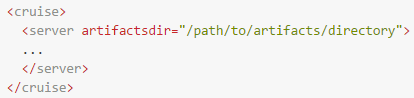
\includegraphics[scale=0.7]{images/ArtifactsDir.png}
            \end{center}
            \caption{Externalisation des artefacts dans GoCD}
            \label{ArtifactsDir}
          \end{figure}

          \paragraph{Configurer l'externalisation des données dans notre Playbook} Dans notre objectif de mettre en place un PIC intégralement « codé » nous devons automatiser cette externalisation via notre Playbook. Dans notre rôle GoCD, nous devons ajouter deux nouvelles tâches qui auront pour but de modifier le fichier de configuration de notre serveur d'Intégration Continue afin qu'il prenne en compte l'externalisation des données.

        \subsection{Architecture et fonctionnement de la PIC}
        Avec cette première version Cloud de notre plate-forme d'Intégration Continue notre serveur GoCD est hébergé durablement dans une Instance EC2 du le Cloud d'Amazon Web Services. L'intégralité de ses données (configuration et artefact) est stockée dans un Bucket S3 afin de pérenniser ces ressources. La création de l'Instance, le déploiement de GoCD et sa configuration sont codés et gérés par Ansible, notre outil de provisionning.\\

        Comme avec la version locale, les développeurs déclenchent l'exécution d'un pipeline de déploiement lors d'un push sur Github. Les utilisateurs peuvent directement intéragir avec GoCD par le biais de son interface web (Voir Figure \ref{PICv2}).\\

        \begin{figure}
          \begin{center}
            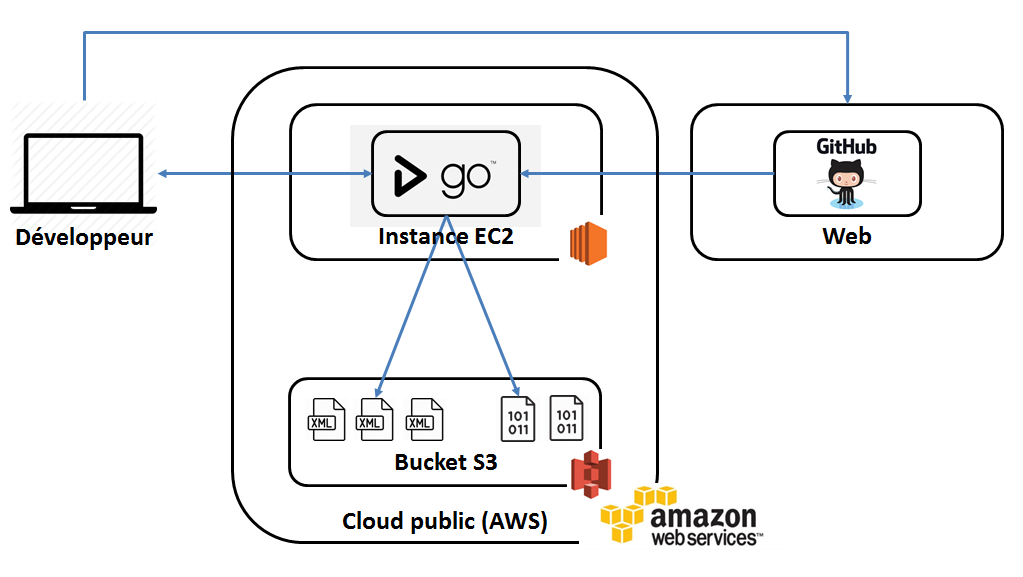
\includegraphics[scale=0.5]{images/PICv2.png}
          \end{center}
          \caption{Schéma de la seconde version de notre PIC - Cloud I}
          \label{PICv2}
        \end{figure}

      \section{Amélioration de la plate-forme d'Intégration Continue en se basant sur le principe du Cloud des instances à la demande}
      Le pilier du Cloud « Infrascture As Code » couplé à un démarrage rapide des instances garanti par les fournisseurs de Cloud apporte une évolution dans la gestion des serveurs au sein des entreprises; les serveurs sont vus comme des consommables que l'on crée et détruit en fonction des besoins. Pour exemple, les instances hébergeant les applications internes d'une entreprise (uniquement utilisé par ses collaborateurs) peuvent être détruites en fin de soirée et relancé au petit matin, dû fait de leur non-utilisation la nuit. Cette nouvelle méthodologie permet de réduire les coûts d'infrastructure tout en garantissant un environnement propre et homogène à nos applications.\\

      Selon les phases d'avancement de notre projet le code source évolue différemment - une évolution forte lors de sa phase de développement et faible lors de sa maintenance applicative - ce qui entraine une utilisation non-homogène de notre PIC. De plus, si notre équipe de développement est exclusivement composée de développeurs travaillant selon le même fuseau horaire la sollicitation de notre serveur d'Intégration Continue lors de sa phase de développement n'est pas non plus également réparti avec une demande forte en journée et quasi nulle la nuit. Le principe d'instance à la demande peut tout à fait être utilisé dans notre cas de notre plate-forme d'Intégration Continue.\\

        \subsection{Ansible notre provisionneur d'instance}
        Dans la section précedente nous avons vu comment Ansible (Voir la section~\ref{Ansible}), un outil de provisionning, pouvait automatiser la création et la configuration de notre serveur d'Intégration Continue dans le Cloud. Nous allons réutiliser ce procédé pour nos instances à la demande.\\

        La solution d'instance à la demande transforme la précedente architecture de notre PIC (Voir Figure \ref{PICv2}). Notre serveur d'Intégration Continue ne sera plus composé d'un logiciel d'Intégration Continue mais d'Ansible, notre provisionneur d'instance qui sera chargé de créer et détruire les instances éphémères qui hébergeront GoCD. Nous aurons ainsi une instance Ansible qui gérera une multitude de serveur d'Intégration.

        \subsection{Le cycle de vie d'une instance hébergeant notre serveur d'Intégration Continue}
        Maintenant que nous avons défini nos instances GoCD comme étant à la demande et éphémère, se pose la question du cyle de vie de ces instances; quand Ansible doit-il créer et détruire un serveur GoCD?\\

          \subsubsection{Une instance à chaque commit sur le serveur de contrôle de code source}
          La première approche naïve, et la plus simple, est de demander à Ansible de provisioner un serveur d'Intégration Continue à chaque fois qu'un développeur pousse son code dans le référentiel de code source et de tuer l'instance à la fin du pipeline de déploiement. Simple, cette solution n'est cependant pas optimal. Rappelons-nous que certaines équipes de développement effectuent plus de cinquante déploiements par jour, soit plus d'un déploiement toutes les dix minutes. Multiplié par le nombre de projet géré par notre PIC, nous arrivons à un nombre de provisionnement considérable géré par une unique instance Ansible, impactant ainsi ses performances.

          \subsubsection{Une instance par cycle de développement}
          La seconde approche pour gérer le cycle de vie de nos instances GoCD est de considérer le cycles de notre application et d'allouer un serveur d'Intégration Continue à chaque phase de développement. Notre serveur GoCD serait ainsi disponnible durant toutes la période de développement et tué lors des périodes de non activités. Le principe d'instance à la demande est respecté mais très peu utilisé.

          \subsubsection{Une instance par jour}
          Dans le cas ou l'intégralité de l'équipe de développement travaille selon le même fuseau horaire nous pouvons définir une politique d'instance journalière lors des cycles de développement. L'instance GoCD serait provisionnée le matin lors du premier commit et détruite chaque soir.

          \subsubsection{Une instance adaptée}
          La dernière approche, et la plus optimisée, s'adapte au besoin de l'équipe de développement en détruisant l'instance GoCD après une période d'inactivité de l'ordre de l'heure (définie par l'équipe). Le principe de l'instance à la demande est ainsi optimisé et garanti une infrasctructure à moindre coût.

        \subsection{Automatiser l'intelligence de notre infrastructure}
        Ansible, quoique très puissant, ne peut gérer le cycle de vie de nos instances GoCD, ne possédant pas de mécanisme d'écoute d'évènement. Il nous faut donc ajouter un middleware\footnote{Middleware: logiciel tiers créant un réseau d'échange entre différentes applications.} entre notre référentiel de code source et notre outil de provisionning afin que ces derniers puissent communiquer.\\

          \subsubsection{Un middleware d'écoute}
          Nous avons vu précédemment que notre référentiel de code source communiquait avec notre serveur d'Intégration Continue via des agents ou via le mécanisme de Webhooks (Voir la section~\ref{Repository}). Ansible, actuellement la seule entité présente de façon durable dans notre PIC, ne possède aucune fonctionnalité citées ci-dessus. La communication entre Github et Ansible est donc impossible. Nous devons ainsi ajouter un outil d'écoute capable de lancer automatiquement et intelligemment des scripts.\\

          La première approche, la plus intuitive mais la plus coûteuse et la moins maintenable, serait de développer un petit outil interne. Ca a été l'approche effectuée par Github pour sa propre plate-forme d'Intégration Continue. Cependant devant l'engouement et le succès de son outil Github a fait évoluer cette outil comme une des pierres angulaires de sa PIC et a décider de publier son outil afin d'en faire standard.

          \subsubsection{Hubot le robot de votre entreprise}\label{Hubot}
          Hubot est un outil d'automatisation de script (CoffeeScript) qui se synchronise avec des services de chat tel que Slack ou HipChat (nous verrons l'utilité de cette fonctionnalité ultérieurement). Initialement développé par Github, Hubot est aujourd'hui un projet open source. Standardisés, les scripts sont partageables et disponibles sur Github.\\

          Dans un premier temps notre robot Hubot doit être capable de recevoir des notifications de Github (ou de tout autre référentiel de code source) et d'exécuter un script Ansible en fonction du cycle de vie de notre serveur d'Intégration Continue. Github et la communauté, très active, propose un script de notification de Github via les Webhooks ainsi qu'un script exécutant les Playbooks d'Ansible. De notre côté nous devons développer un troisième script qui, appelé par le script de Github, exécutera le script d'Ansible en fonction de la gestion du cycle de vie de l'instance de GoCD vu précédemment (Voir figure \ref{HubotScripts1}).\\

          \begin{figure}
            \begin{center}
              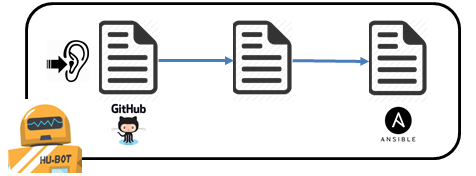
\includegraphics[scale=0.7]{images/HubotScripts1.png}
            \end{center}
            \caption{Hubot - Gestion des notifications de Github}
            \label{HubotScripts1}
          \end{figure}

      \subsection{La chatroom, le point d'entrée de notre plate-forme d'Intégration Continue}
      Un des bénéfices primaires de l'Intégration Continue est d'améliorer la visibilité du projet en fournissant des informations en temps réels sur l'état des builds ainsi que des rapports sur la qualité du code source. En faisant évoluer notre serveur GoCD en instance à la demande nous perdons l'aspect permanent de cette visibilité - si l'instance GoCD n'est pas déployée et active, nos utilisateurs ne disposent d'aucun point d'entrée sur notre PIC. Nous devons ainsi mettre à la disposition des utilisateurs de l'Intégration Continu une interface permanente afin qu'ils puissent intéragir avec notre serveur.\\

      Cette nouvelle interface doit respecter quatre grands principes si nous voulons qu'elle ajoute de la valeur à notre plate-forme d'Intégration Continue:\\

      \begin{itemize}
        \item la permanence: pour répondre à la contrainte du serveur GoCD à la demande,
        \item l'omniscience: toutes les informations sur l'Intégration Continue doivent y figurer,
        \item l'intérêt: l'interface doit avoir un intérêt autre que celle de GoCD,
        \item l'évolutivité: afin d'y intégrer de nouvelles fonctionnalités.\\
      \end{itemize}

        \subsubsection{Les principes fondamentaux de notre point d'entrée}
          \paragraph{La permanence} Nous avons déjà évoqué précédemment la qualité de permanence - indispensable - du point d'entrée de notre PIC. Les informations créés et stockées sur notre serveur d'Intégration Continue doivent être disponible à tout moment et récupéré facilement. Notre interface devra donc être déployé sur un serveur pérenne, issu de nos serveurs privés ou du Cloud, accessible par tous et de partout.
          Dans notre cas, le point d'entrée sera installé sur notre serveur hébergeant Ansible et Hubot mais il pourra tout aussi bien être installé sur un serveur distant ou fonctionner en mode SaaS (Voir l'annexe \ref{CloudComputingAnnexe}).

          \paragraph{L'omniscience} Notre point d'entrée, et notre unique correspondant avec notre serveur, doit être capable de restituer l'intégralité des informations produites par la PIC. Cette restitution doit être claire, lisible et graphique.
          GoCD stocke la totalité de ses informations sous forme de fichier XML. Notre interface devra être capable d'interpréter le XML et de le retranscrire graphiquement.

          \paragraph{L'intérêt} Notre interface, outre le fait qu'elle doive implémenter des services analogues à celle proposé par GoCD, doit proposer de nouvelles fonctionnalités ayant pour but d'améliorer l'Intégration Continu.
          Un des points faibles des plate-formes d'Intégration Continue est la notion de communication - qu'elle soit entre le serveur et les utilisateurs ou entre les utilisateurs eux-mêmes. La PIC induit à une communication asynchrone souvent mal gérée. La communication entre les acteurs d'un même projet est très importantes. L'intérêt de notre point d'entrée serait de fournir un mécanisme de communication asynchrone et tracée car les conversations que l'on a autour du code sont aussi importantes que le code lui-même. L'idée serait d'avoir au même endroit que notre produit fini (le code) la « recette » qui nous a permis d'y arriver.

          \paragraph{L'évolutivité} L'Intégration Continue est un concept jeune qui ne cesse d'évoluer. Notre interface devra être capable d'intégrer et de centraliser les fonctionnalités futures qui seront présentes dans les futures implémentations des plate-formes d'Intégration Continue.
          Devant l'inconnue de ces futures fonctionnalités, le meilleur outil que nous pouvons utiliser les intégrer reste la ligne de commande. La ligne de commande permet aux utilisateurs d'un service informatique d'exécuter une commande, accompagnée de ces arguments, prédéfinie, l'évolutivité est ainsi infinie.

        \subsubsection{Le choix de notre point d'entrée: la chatroom}
        Cette section va être consacré au choix de l'outil que nous allons utiliser comme point d'entrée de notre PIC. Commençons par faire un petit récapitulatif des fonctionnalités que doit proposer cet outil:\\

        \begin{itemize}
          \item un mécanisme de réprésentation des informations de l'Intégration Continue,
          \item un mécanisme de ligne de commande pour intéragir avec notre serveur,
          \item un mécanisme de communication asynchrone.\\
        \end{itemize}

        Maintenant rappelons nous qu'Hubot a été designé par les équipes de Github pour s'intégrer à des plate-formes de communication collaborative tel que Slack et HipChat (Voir la section \ref{Hubot}). En étudiant ces outils nous remarquons qu'ils remplissent les trois fonctionnalités essentielles de notre point d'entrée; de part leur nature ils fournissent une communication asynchrone et ils disposent d'une interface graphique pour la représentation des informations ainsi qu'une zone de saisie de texte pour le mécanisme de ligne de commande (Voir figure {\ref{Slack}}). De plus principes des plate-formes de travail collaborative est déjà fortement présent au sein des équipes de travail, l'utilisation d'un tel outil n'est ainsi déconcertant pour les collaborateurs. Nous allons donc nous appuyer cet outil pour notre point d'entrée.\\

        \begin{figure}
          \begin{center}
            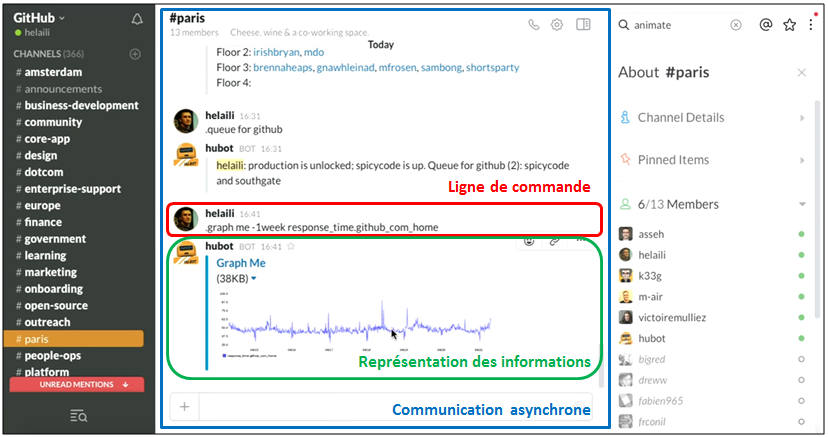
\includegraphics[scale=0.5]{images/Slack.png}
          \end{center}
          \caption{Slack - Example d'une chatroom au sein des équipes de travail à Github}
          \label{Slack}
        \end{figure}

        Les plate-formes de communication collaborative, très à la mode ces dernières années, sont fortements présentent sur le marché (Slack, HipChat, Mattermost, ...). Le choix de telle ou telle plate-forme dépendra essentiellement de votre entreprise, mais toutes offrent globalement les mêmes services. Il vous faudra juste vérifier la disponibilité d'un adaptateur Hubot pour que ce dernier puisse communiquer avec. Dans le cas contraire libre à vous de développer et de soumettre votre plugin à la communauté. Dans notre cas d'une plate-forme d'Intégration Continue open-source nous allons nous tourner vers Mattermost, une alternative open source à Slack.

        \subsubsection{Les communications}
          \paragraph{Une communication asynchrone entre les collaborateurs}
          La communication asynchrone est souvent négligée dans les entreprises. Sans traçabilité, archivage et partage des conversations de nombreuses décisions sont remises en cause ou non appliquées. De plus avec l'internalisation des organisations des équipes de travail se trouvent distribuées à travers la planète, sur des fuseaux horaires différents, cependant il faut qu'ils puissent travailler ensemble sans se voir, sans appels vocals ou visuel. Il leurs faut donc un mode de fonctionnement qui leur permet de collaborer sans perte de temps et d'efficacité. La communication asynchrone répond à ces deux problématiques.

          \paragraph{Une communication par ligne de commande entre les collaborateurs et Hubot}
          Outre communiquer avec les autres collaborateurs, Mattermost permet de communiquer avec Hubot, notre robot d'Intégration Continue. Cette communication nous permet d'avoir un point d'entrée sur notre PIC ainsi que d'y exécuter diverses actions, par le biais de lignes de commandes. Ces dernières, écrites et interprétées dans le flux de message, sont transmisent à Hubot grâce au connecteur afin de déclencher l'exécution des scripts responsable du traitement de la tâche. De plus, le mécanisme d'asynchronité est aussi valable pour les lignes de commandes et ses résultats.

          \paragraph{Une communication par API entre Hubot et GoCD}
          GoCD, comme la plupart des serveurs d'Intégration Continue, fournit une API afin que des applications tierses puissent intéragir avec lui. Cette API, se reposant sur le protocole HTTP (HyperText Transfer Protocol) - le protocole de communication client-serveur développé pour le World Wide Web - et sur l'architecture REST (Representatinal State Transfer) - architecture de communication pour les systèmes hypermédias distribués - expose l'ensemble de ses services sous la forme d'URL permettant ainsi à Hubot de les consommer.

        \subsubsection{Mise en place de la plate-formes de communication collaborative}

          \paragraph{L'automatisation de son déploiement}
          Dans notre solution de PIC nous hébergeons Mattermost dans notre instance fixe contenant Ansible et Hubot. Comme tous les autres outils utilisés jusqu'à maintenant dans notre plate-forme d'Intégration Continue, la mise en place, la configuration et la maintenance de Mattermost doit être automatisé par le code. Nous devons donc ajouter un nouveau rôle dans notre Playbook responsable de notre plate-formes de communication collaborative. Ansible Galaxy, le dépôt de Playbook d'Ansible, propose un artefact pré-configuré pour le déploiement de Mattermost.

          \paragraph{L'archivage des données}
          Mattermost stocke l'intégralité de ses données dans une base de données SQL (MySQL ou PostgreSQL). Plutôt que d'héberger notre propre base de données et d'assurer nos propres mécanismes de réplication des données nous préférons faire appel au service de gestion des bases de données de notre fournisseur de Cloud: Relational Database Service (RDS). Ce dernier permet d'installer, de gérer et de mettre à l'échelle facilement une base de données relationnelle dans le Cloud. Les tâches fastidieuses d'administration et de maintenances des bases sont déléguées à Amazon Web Services. Nous assurons ainsi la pérennité des données de notre plate-forme de travail.

          \paragraph{L'organisation de travail}
          Les plate-formes de communication collaborative s'organisent autour de salons - les chatrooms. Ils peuvent être publics et donc visible par l'ensemble des collaborateurs ayant accès à l'outil ou privés pour restreindre l'accès à votre channel (sous forme d'invitation). Du fait de son caractère sensible et de son accès aux différents serveurs de production, la chatroom responsable du point d'entrée de votre serveur d'Intégration Continue devra être privée et uniquement accueillir votre équipe de travail.

        \subsubsection{Les fonctionnalités}
        Mattermost, notre interface utilisateur par ligne de commande, couplé à Hubot, notre gestionnaire de scripts, offre une infinité de fonctionnalités. Nous pouvons par exemple trouver sur internet des scripts permettant de commander des pizzas, de connaître l'emplacement des food-trucks à proximité ou encore de localiser vos collègues de travail, tout cela depuis une chatroom. Mais qu'elles sont les fonctionnalités, utiles à l'Intégration Continue, que nous pouvons intégrer à notre PIC?

          \paragraph{L'intégration} Le but premier de l'Intégration Continue étant comme son nom l'indique l'intégration d'un morceau de code dans l'application et son déploiement, la première fonctionnalité à mettre en place est le déclencheur du pipeline de déploiement. Nous avons vu précédemment que l'exécution de ce workflow de déploiement était déclenché par un Webhook lors de la synchronisation d'un code source local avec le gestionnaire de contrôle de version. Nous devons ainsi intégrer une commande permettant de pousser son code au niveau du référentiel partagé. Pour respecter la méthodologie des branches (Voir la section \ref{SCM}) cette commande prendra en compte en premier paramètre la branche de travail cible. Une fois le code envoyé aucune autre action manuelle n'est requise, le Pipeline GoCD s'exécute automatiquement. Un retour en direct de l'avancé de votre Pipeline est fortement recommandé. En cas d'échec Mattermost doit fournir un apercu graphique des différents rapports liés au non succès d'une Task afin que le problème soit résolu le plus rapidemment possible.

          \paragraph{Le déploiement} Une fois l'intégration effectuée nous devons déployer la nouvelle version sans nouvelle action de la part du développeur. Nous allons donc ajouter un paramètre à notre précédente commande désignant les serveurs cibles de notre déploiement. L'ensemble des environnements sont configurés au niveau d'Hubot et dispose de groupe et d'alias, les développeurs n'ont ainsi pas l'obligation de connaitre l'URL du serveur, ils ont juste à indiquer le nom d'environnement souhaité.
          La commande d'intégration et de déploiement sera donc composée d'un nom - « /hubot deploy » - et de deux paramètres, la branche du repository cible et l'alias de l'environnement de déploiement (Voir la Figure \ref{SlackDeploy}).
          Dans le cas où nous ne désirons déployer notre application que sur certains serveurs de notre environnement, le second paramètre - celui de l'environnement - devra être renseigné sous la forme d'une expression régulière comprenant le nom de l'environnement et l'alias des serveurs.

          \begin{figure}
            \begin{center}
              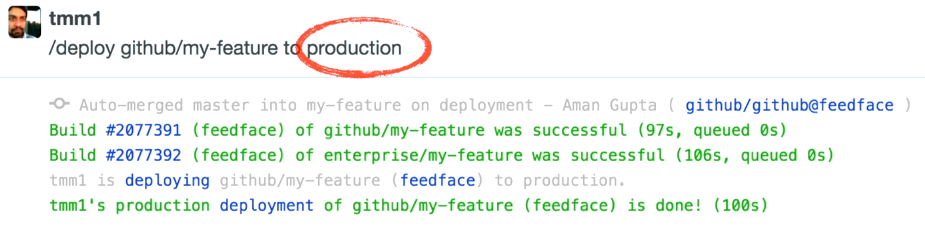
\includegraphics[scale=0.5]{images/SlackDeploy.png}
            \end{center}
            \caption{Exemple d'une commande de déploiement dans Slack}
            \label{SlackDeploy}
          \end{figure}

          \paragraph{La queue de déploiement} Pendant les heures de pointe de travail, plusieurs développeurs essaient souvent de déployer leurs changements simultanément dans le même environnement. Pour éviter toute confusion et donner une chance à tous de déployer, nous ajoutons à Hubot une file d'attente de déploiement. Les développeurs désirant déployer doivent ainsi s'enregister auprès d'Hubot et attendre leur tour. Cette nouvelle fonctionnalité s'appuie sur trois commandes.
          La première des trois - « /hubot queue » - permet de connaitre l'état en cours de la file de déploiement de l'environnement passé en paramètre. Hubot nous renverra la liste des développeurs en attente de déploiement.
          La seconde commande - « /hubot queueme » - permet aux développeurs de s'enregister dans la queue de déploiement de l'environnement passé en paramètre.
          La troisième commande - « /hubot unqueueme » - permet aux développeurs présents dans la file de l'environnement passé en paramètre de s'y retirer.

          \paragraph{Le verrou de déploiement} Toujours dans une optique de déploiement simultané sur un même environnement nous devons implémenter une fonctionnalité de verrouillage sur la branche déployée afin que l'intégralité des tests soient effectué avant le déploiement d'une nouvelle version. Pour cela nous ajoutons à notre script Hubot de déploiement une instruction chargée de gerer le verrou des environnements.

          \paragraph{La maintenance applicative} La plupart des équipes de développement disposent d'un outil de suivi de bugs afin de tracer et corriger les disfonctionnements de leurs applications liées aux erreurs de développement. Qu'il fonctionne sur le principe de carte (Jira) ou d'issue (Github) notre chatroom doit être en capacité de retranscrire le bug dans le flux de conversation du projet. Le bug est ainsi directement pris en compte par l'équipe de développement et corrigé rapidemment. Les développeurs doivent aussi être en mesure de clore les cartes ou issues une fois celle-ci traité. Pour cela nous allons ajouter une troisième paramètre à notre commande de déploiement spécifiant l'identifiant du disfonctionnement retourné par l'outil de suivi de bugs.

          \paragraph{La sécurité} Un des points importants au sein des services informatiques est la sécurité des serveurs. Avec un script Hubot, nous pouvons gérer l'accés aux différents serveurs en fonction des collaborateurs selon un principe d'autorisation, seules les personnes autorisées peuvent effectuer des actions sur les environnements. De plus notre plate-forme d'Intégration Continue garantie la confidentialité des chaînes de connexion et des mots de passe des serveurs. L'intégralité des données de connexion aux environnements et l'accès à ces derniers étant géré par Hubot, la perte ou la fuite de ces informations critiques est ainsi minimisée.

      \subsection{Architecture et fonctionnement de la PIC}
      Dans sa version finale, notre plate-forme d'Intégration Continue est composé d'un serveur permanent « maître » dans le Cloud Amazon Web Services - hébergeant Mattermost (outil de communication asynchrone) le point d'entrée de notre PIC, Hubot (outil d'exécution de scripts) notre robot intelligent et Ansible notre outil de provisionning d'instance - et d'instances éphémères « esclave », elles aussi dans le Cloud AWS, qui accueillent notre serveur d'Intégration Continue GoCD.\\
      Du point de vue fonctionnement, nos équipes de travail intéragissent indirectement avec le serveur d'Intégration par le biais de lignes de commande via les chatrooms présentent au sein de la plate-forme de communication et Hubot (Voir Figure \ref{PICv3}).\\
      Comme dans notre version précédente, l'intégralité des déploiements, « maître » comme « esclave », est automatisé et géré par Ansible.

      \begin{figure}
        \begin{center}
          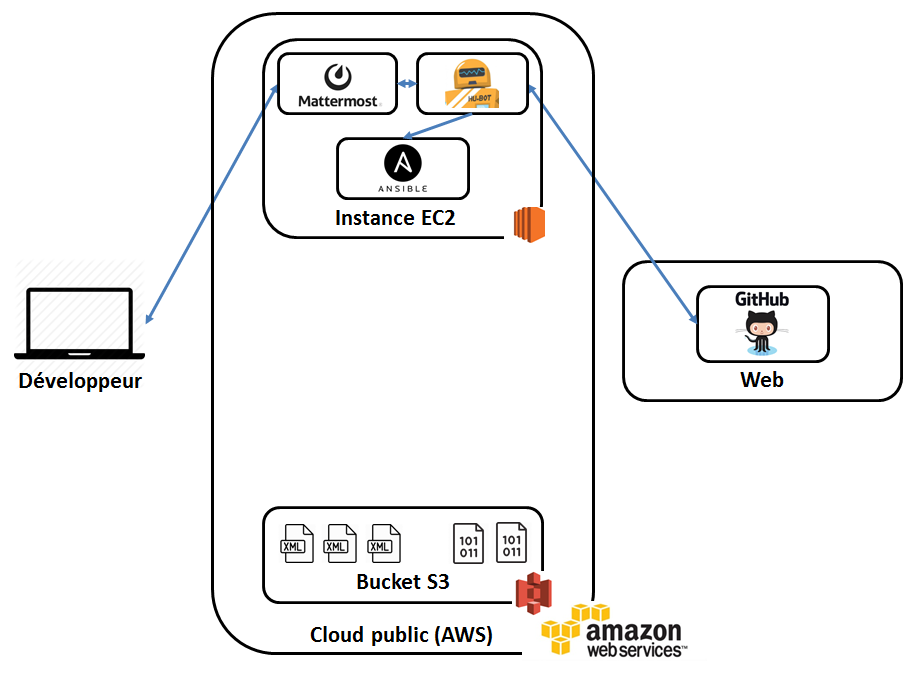
\includegraphics[scale=0.5]{images/PICv3.png}
        \end{center}
        \caption{Schéma de la troisième version de notre PIC - Cloud II}
        \label{PICv3}
      \end{figure}

      \section{Aller plus loin}
      Avant de poursuivre avec l'ultime chapitre de ce mémoire qui a pour vocation de proposer des axes d'améliorations et de nouvelles fonctionnalités à notre solution, nous allons faire un petit récapitulatif des outils, des caractéristiques et des fonctionnalités de notre plate-forme d'Intégration Continue. Pour les outils, nous avons utilisé:\\

      \begin{itemize}
        \item un serveur d'Intégration Continue (GoCD),
        \item un référentiel de code source (Git/Github),
        \item un fournisseur de Cloud (Amazon Web Service),
        \item un provisionneur d'instances (Ansible),
        \item un exécuteur de scripts (Hubot),
        \item une plate-forme de communication asynchrone (Mattermost).\\
      \end{itemize}

      Du côté des caractéristiques notre solution est:\\

      \begin{itemize}
        \item multiplate-forme (Windows et Linux),
        \item multi-langage (.NET, JAVA/J2EE, Javascript, ...),
        \item multi-référentiel de code source (Git, TFS, SVN, ...),
        \item open source,
        \item automatisé,
        \item « First Class »,
        \item « Infrasctucture As Code »,
        \item à la demande.
      \end{itemize}

      Et a pour fonctionnalité:\\

      \begin{itemize}
        \item l'intégration,
        \item l'exécution des analyses statiques du code,
        \item la build,
        \item l'exécution des tests,
        \item la création de rapports,
        \item la création de documentation,
        \item le déploiement,
        \item la maintenance,
        \item la sécurité.\\
      \end{itemize}

      Nous constatons que notre solution répond à l'intégralité des critères de l'Intégration Continue vu en première partie de ce mémoire (Voir le Chapitre \ref{ContinousIntegration}). Mais de nombreuses autres problématiques liés aux cycles de vie des applications et aux développements en lui-même peuvent être greffées à notre plate-forme. Nous allons en voir quelques unes et essayer d'offrir des pistes de reflexion quant à leur intégration.

      \subsection{Les analyses, le monitoring et les alertes}
      Il peut s'avérer très intéressant pour les équipes de travailler avec des rapports d'analyses controllant les performances, les charges, les disponibilités, l'utilisation des fonctionnalités, etc de leurs applications. Les applications de monitoring perforent le marché des solutions informatiques et sont de plus en plus sollicité par les organisations. Il peut s'avérer utile d'intégrer des commandes à notre plate-forme d'Intégration Continue permettant d'avoir une représentation graphique des diverses analyses. Au vue des nombreux acteurs de monitoring et des solutions développées en interne il est difficile de conjecturer sur une solution générique, vous devrez sans doute développer votre propre script Hubot.\\

      Mais plus que monitorer pour monitorer les équipes de travail désirent surtout recevoir des alertes lorsque les seuils fixés sont atteints et que le fonctionnement de l'application devient critique. Votre script devra être capable d'écouter - c'est la solution à privilégier - ou interroger à des intervalles de temps régulier vos outils de monitoring. Les développeurs seront ainsi rapidement et efficacement prévenus des dysfonctionnements de l'application.

      \subsection{La remontée automatique des dysfonctionnements lié au code}
      Les dysfonctionnements d'une application peuvent être de natures diverses; nous avons les bugs techniques, les bug liés au code, les bugs d'utilisation... Cependant ils ont une chose en commun, ils doivent être résolus rapidemment sous peine d'endommager le fonctionnement de l'application. Principalement les bugs impactants les developpeurs sont ceux liés au code, qu'ils soient fonctionnels, de conception ou lié au langage. Si l'application dispose d'une remontée d'erreur efficace, la source du dysfonctionnement (trace d'appel ou « stack trace ») est archivée dans un fichier de logs et permet ainsi aux équipes d'en comprendre la provenance et de le corriger en un rien de temps. Nous constatons malheureusement que le temps de correction d'un bug est anormalement élevé, ce qui favorise sa reproduction. En étudiant son cycle de vie (celui de la correction du bug) nous remarquons que ce temps n'est pas dû à la correction du bug lui-même mais en sa prise de connaissance de la part des développeurs. Il peut être alors très utile de disposer d'un service de remontée automatique pour les dysfonctionnements lié au code directement dans la chatroom de l'équipe. La remontée pourrait se faire sous forme d'alerte, indiquant la stack trace et le nom du dernier développeur ayant modifier la portion de code impactée.\\

      Au niveau de la mise en place nous partons sur l'idée d'un ETL\footnote{Extract-Transform-Load: technologie informatique intergicielle (middleware) permettant d'effectuer des synchronisations massives d'information d'une source de données vers une autre.} destiné aux logs tel que Logstash (open source) qui écouterait les fichiers de logs et transférerait les nouveaux logs d'erreurs à Hubot. Ce dernier n'aurait plus qu'à alerter Mattermost.

      \subsection{Un dépôt de plate-forme d'Intégration Continue}
      L'automatisation du provisionning, du déploiement et de la configuration de notre plate-forme d'Intégration Continue est étroitement lié au système d'exploitation de l'environnement et du langage de programmation de l'application.
